% Asset ID: A21ParametricEquationsTikZ-006
% Source: Transcript modelling section; PowerPoint modelling slide; CCEA A21-CG-LO002.
% Related lesson section: Worked Example 7; Modelling.
% Purpose: Show time as a parameter in two-dimensional motion.

\documentclass[tikz,border=8pt]{standalone}
\usepackage{amsmath}
\usetikzlibrary{arrows.meta,angles,quotes}
\begin{document}
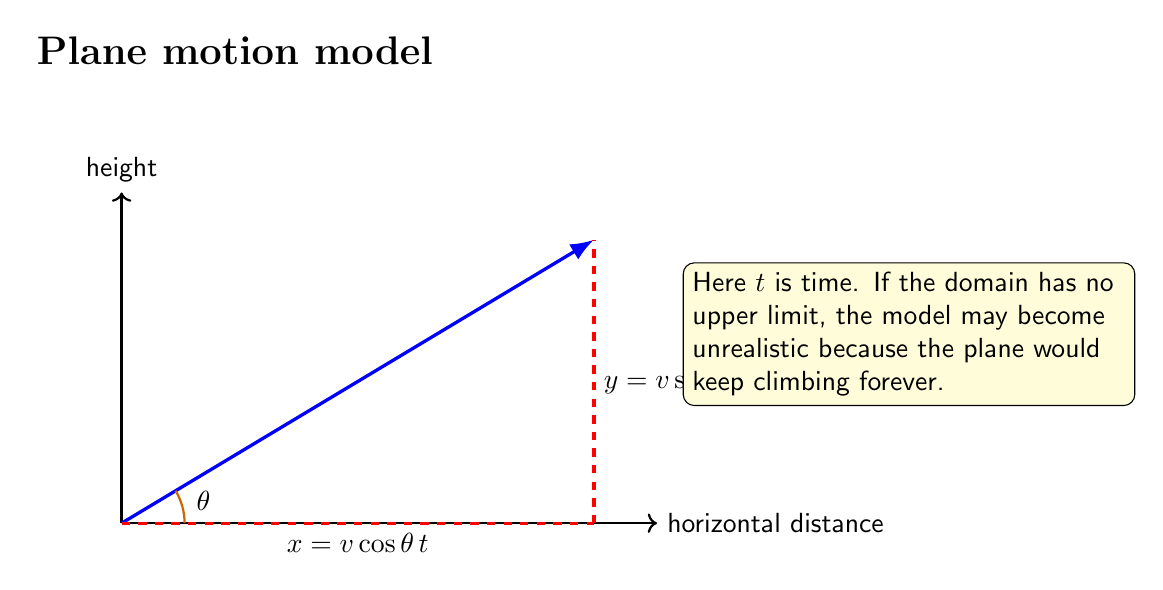
\begin{tikzpicture}[font=\sffamily]
\node[anchor=west, font=\bfseries\Large] at (-6.2,4.0) {Plane motion model};
\coordinate (O) at (-5,-2);
\coordinate (X) at (1,-2);
\coordinate (P) at (1,1.6);
\draw[thick,->] (O) -- (1.8,-2) node[right] {horizontal distance};
\draw[thick,->] (O) -- (-5,2.2) node[above] {height};
\draw[very thick,blue,-{Latex[length=3mm]}] (O) -- (P);
\draw[very thick,red,dashed] (O) -- (X);
\draw[very thick,red,dashed] (X) -- (P);
\node[below] at (-2,-2) {\(\displaystyle x=v\cos\theta\,t\)};
\node[right] at (1,-0.2) {\(\displaystyle y=v\sin\theta\,t\)};
\pic[draw=orange!80!black, thick, angle radius=0.8cm, "$\theta$", angle eccentricity=1.35] {angle=X--O--P};
\node[draw, rounded corners, fill=yellow!15, text width=5.5cm] at (5,0.4) {Here \(t\) is time. If the domain has no upper limit, the model may become unrealistic because the plane would keep climbing forever.};
\end{tikzpicture}
\end{document}
